\chapter{Мониторинг дрейфа морского льда и айсбергов на основе результатов анализа SAR"~изображений} \label{chapt4}

В данной главе описывается применение гидродинамическая модель дрейфа айсбергов, в рамках разработанной технологии ледового мониторинга в Карском море на основе данных автоматизированного анализа SAR"~изображений, а также в контексте усовершенствования ледового мониторинга в Баренцевом море.

Мониторинг динамических характеристик льда "--- дрейфа и деформации, рассматривается на примере разработанной технологии автоматической обработки последовательных спутниковых SAR"~изображений.

\section{Моделирование дрейфа айсбергов как часть ледового мониторинга в Западной Арктике} \label{sect4_1}

Айсберги наблюдаются в большинстве районов морей Западной Арктики, и встреча с ними является одной из наиболее реальных и опасных угроз для судов и морских производственных объектов~\cite{Mironov_Smirnov_Iceberg_2015}. В последние годы, в связи с активными работами по освоению нефтегазовых месторождений на шельфе Баренцева и Карского морей вопрос предотвращения айсберговой угрозы становится особенно острым. Ледовые угрозы относятся к категории управляемых, поскольку существует возможность воздействовать на тяжёлые льды и айсберги с помощью ледоколов и других средств. Это осуществляется с помощью системы управления ледовой обстановкой (УЛО) или ледового менеджмента. Ледовый мониторинг, включающий наблюдения, оценку и прогноз возможных изменений ледовых условий является ключевым компонентом УЛО.

Для исследования распространения айсбергов и закономерностей их дрейфа 
используются различные методы наблюдений, такие, как спутниковый мониторинг, 
аэрофотосъемка с вертолета или беспилотного летательного аппарата, установка 
радиомаяка на айсберг. Значительный опыт мониторинга айсбергов имеется у ледовых служб Канады, Дании и Норвегии. Радиолокационные спутниковые изображения высокого разрешения позволяют осуществлять обнаружение айсбергов и их мониторинг, аэрофотосъемка айсбергов позволяет получать морфометрические характеристики их верхней поверхности, а с помощью радиомаяков, установленных на их верхнюю поверхность, можно отслеживать траектории перемещения айсбергов. Эти данные необходимы для статистического анализа параметров дрейфа и верификации математических моделей дрейфа айсбергов.

Численное гидродинамическое моделирование может оказать существенную помощь при организации системы ледового мониторинга в Западной Арктике. Гидродинамические модели являются основой прогнозирования движения и трансформации айсбергов, помогают ранжировать источники айсбергов по степени их опасности для исследуемого района. В настоящем разделе описываются возможности применения гидродинамической модели дрейфа айсбергов для оперативного обеспечения морской деятельности на шельфе и для исследовательских работ по оптимизации системы ледового мониторинга в Западной Арктике с использованием данных о местоположении айсбергов, полученных на основе автоматизированного анализа SAR"~данных.

\subsection{Краткое описание модели дрейфа айсбергов} \label{subsect4_1_1}

Уравнение баланса сил, действующих на айсберг, дрейфующий в поверхностном слое воды, запишем в виде:

\begin{equation}
\label{eq:equation4_1}
m{\frac{\vec{\partial W_i}}{\partial t}} = \vec{F_a}+\vec{F_w}+\vec{F_{if}}+\vec{F_p}+\vec{F_C},
\end{equation}
где $\vec{W_i}$ "--- скорость дрейфа айсберга, $m$ "--- его масса, $\vec{F_a}$ "--- сила воздействия ветра, $\vec{F_w}$ "--- сила воздействия течения, $\vec{F_{if}}$ "--- сила воздействия дрейфующего льда, $\vec{F_C}$ "--- сила Кориолиса, $t$ "--- время.

Силу воздействия ветра на айсберг запишем в соответствии с классической квардратической зависимостью от скорости ветра:

\begin{equation}
\label{eq:equation4_2}
\vec{F_a} = \rho_{a}S_{a}C_{a}\left|{\vec{W_a}}\right|\left(\vec{W_a}\right),
\end{equation}
где $\vec{W_a}$ "--- скорость ветра, $\rho_{a}$ "--- плотность воздуха, $S_{a}$ "--- надводная площадь айсберга перпендикулярная направлению ветра, $C_{a}$ "---  эмпирический коэффициент.

Силу воздействия течений на айсберг выразим квардратической зависимостью от разницы скорости течения и дрейфа айсберга:

\begin{equation}
\label{eq:equation4_3}
\vec{F_w} = \rho_{w}S_{w}C_{w}\left|{\vec{W_w}-\vec{W_i}}\right|\left({\vec{W_w}-\vec{W_i}}\right),
\end{equation}
где $\vec{W_w}$ "--- средняя в слое от поверхности до нижней границы айсберга скорость течения, $\rho_{w}$ "--- плотность воды, $S_{w}$ "--- подводная площадь айсберга перпендикулярная направлению среднего течения, $C_{w}$ "---  эмпирический коэффициент.

Силу воздействия дрейфующего льда на айсберг выразим квардратической зависимостью от разницы скорости дрейфа льда и скорости дрейфа айсберга:

\begin{equation}
\label{eq:equation4_4}
\vec{F_{if}} = \rho_{i}S_{if}C_{if}\left|{\vec{W_{if}}-\vec{W_i}}\right|\left({\vec{W_{if}}-\vec{W_i}}\right),
\end{equation}
где $\vec{W_{if}}$ "--- скорость дрейфа льда, $\rho_{i}$ "--- плотность льда, $S_{if}$ "--- площадь айсберга, находящаяся в соприкосновении с дрейфующим льдом и перпендикулярно направлению его дрейфа, $C_{if}$ "---  эмпирический коэффициент.

Силу градиента давления определим через проекцию силы тяжести на горизонтальную поверхность:

\begin{equation}
\label{eq:equation4_5}
\vec{F_{p}} = gm\vec{\nabla}\zeta,
\end{equation}
где $g$ "--- ускорение свободного падения, $\zeta$ "--- превышение уровня моря над невозмущенной поверхностью.

Силу Кориолиса запишем в классическом виде:

\begin{equation}
\label{eq:equation4_6}
\vec{F_{c}} = \Omega m\vec{k}\times \vec{W_i},
\end{equation}
где $\Omega$ "--- угловая скорость вращения, $k$ "--- единичный вектор, направленный вертикально вверх.

Сформулированная задача (\labelcref{eq:equation4_1,eq:equation4_2,eq:equation4_3,eq:equation4_4,eq:equation4_5,eq:equation4_6}) позволяет средствами численного математического моделирования определить скорость, а в дальнейшем и траекторию дрейфа айсберга при известных форсингах. Однако если существует несколько доступных путей получения скорости ветра, то такие параметры, как скорость течения, скорость дрейфа льда и денивеляция уровенной поверхности моря, можно получить только путем их расчета в модели совместной циркуляции вод и льдов. В данном исследовании в качестве такой модели будем использовать AARI"~IOCM~\cite{Kulakov2012}. AARI"~IOCM представляет собой результат объединения трех моделей: трехмерной бароклинной модели циркуляции вод, модели дрейфа ледяного покрова и термодинамической модели морского льда. Модель адаптирована к акватории Северного Ледовитого океана (СЛО) и прилежащей акватории Атлантического океана и имеет пространственное разрешение 13,8 км. Размер сеточной области 440 на 395 точек. По вертикали разрешение переменное, расчет производится на 33 горизонтах. Для описания донной топографии и конфигурации береговой черты использован архив GEBCO. В качестве граничных условий используются среднемесячные среднемноголетние значения расходов 17 основных рек, впадающих в СЛО. Температура и соленость воды из World Ocean Atlas (WOA05) для летнего или зимнего периодов взяты в качестве начальных условий. В качестве внешнего форсинга используются данные об атмосферном давлении на уровне моря и температуре воздуха на высоте 2 м из архива NCEP/NCAR для диагностических расчетов или прогностические данные Европейского центра среднесрочных прогнозов погоды (ECMWF), представленные на сетке $2,5^\circ \times 2,5^\circ$.

Модель была верифицирована по данным радиомаяков ARGOS установленных на айсберги в экспедиции <<Кара"~зима"~2013>>. Результаты расчетов показали, что модель удовлетворительно воспроизводит дрейф айсбергов (рис.~\ref{img:ibg_validation_01}).

\begin{figure}[ht] 
	\centering
	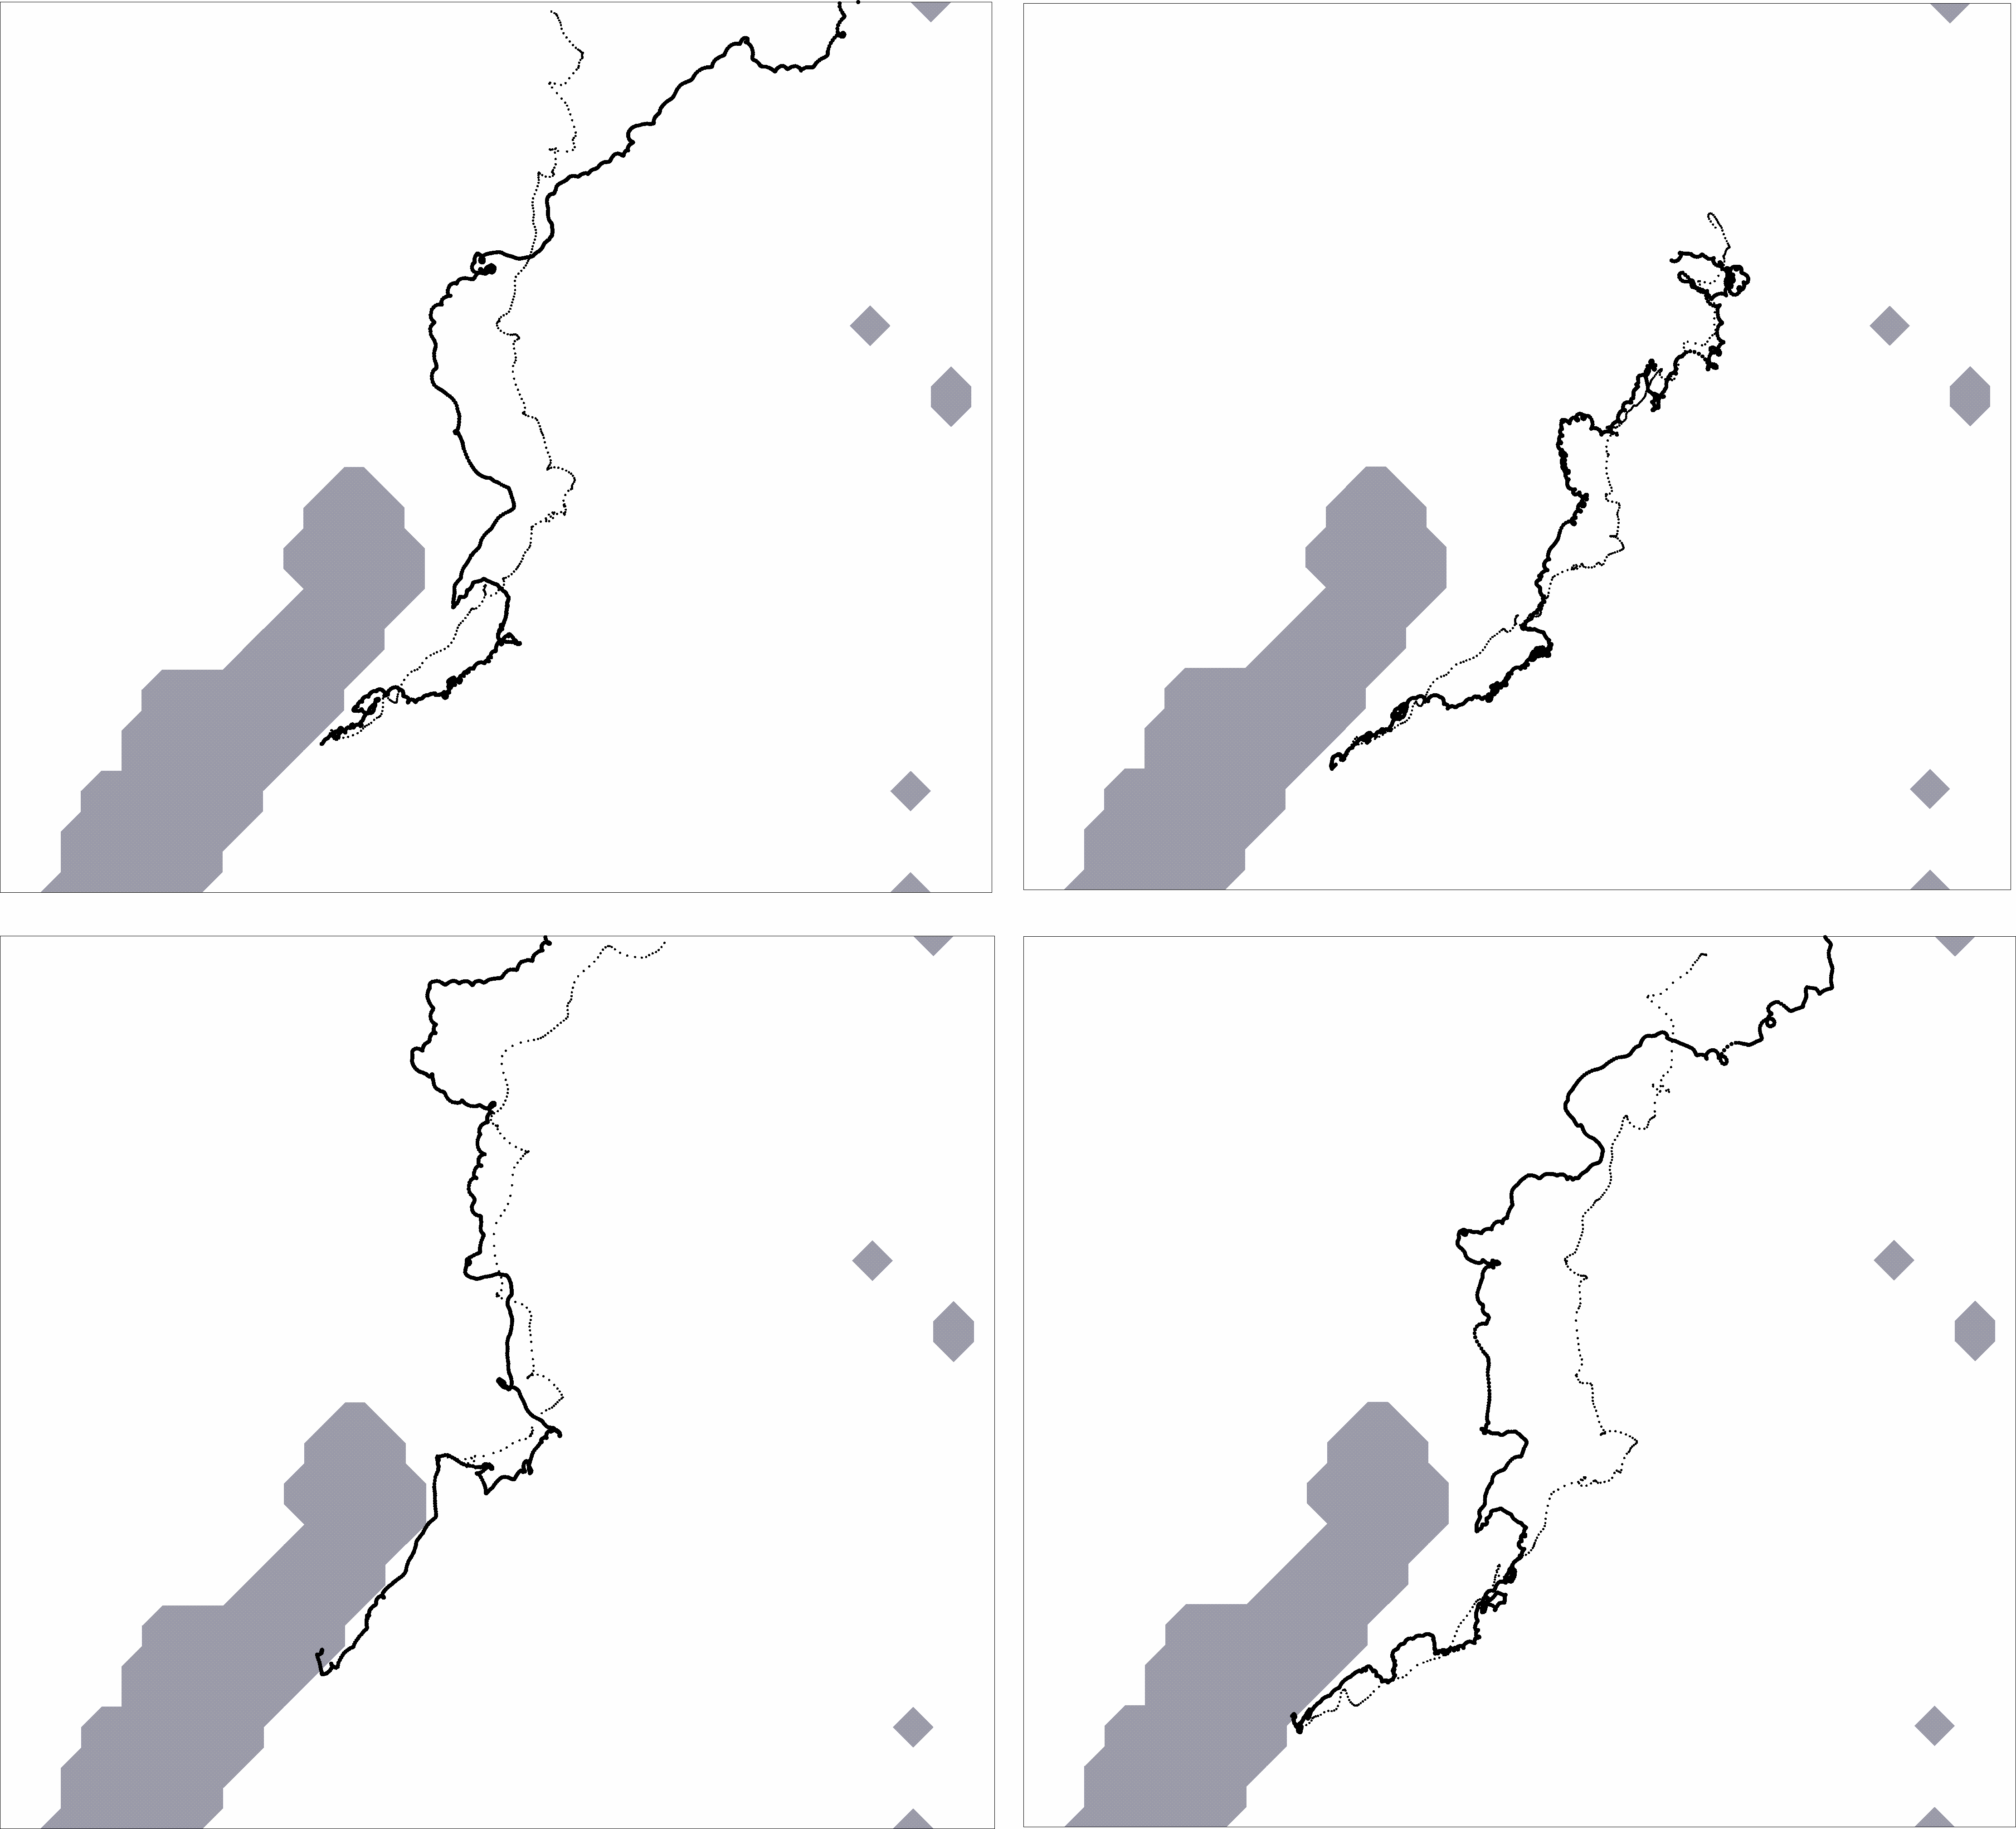
\includegraphics [scale=0.08] {ibg_validation_01}
	\caption{Сопоставление наблюденных (жирная линия) и рассчитанных по модели (тонкая линия) траекторий айсбергов в 2013 г.}
	\label{img:ibg_validation_01}
\end{figure}

\subsection{Обнаружение айсбергов на основе спутниковых радиолокационных данных}
Обнаружение айсбергов с помощью спутниковых радиолокаторов основано на 
том, что обратный РЛ"~сигнал от айсберга, как правило, выше, чем интенсивность 
обратного рассеивания от водной поверхности и ледяного покрова. Принципиальная возможность обнаружения айсбергов на спутниковых радарных изображениях была показана в 1990"~е гг. на примере снимков радиолокатора спутника <<Алмаз"~1>>, на которых уверенно обнаруживались айсберги среди припая и сплошных 
дрейфующих льдов~\cite{Alexandrov1996}. Позднее для мониторинга айсбергов были 
успешно использованы европейские и канадские радиолокационные спутники. Было 
установлено, что обратный РЛ"~сигнал дрейфующего льда существенно изменяется в 
зависимости от возраста, формы, состояния поверхности и других параметров ледяного покрова. Причем вероятность обнаружения айсбергов с помощью спутниковых средств наблюдения зависит от соотношения размера айсберга и пространственного разрешения аппаратуры, формы и степени разрушенности айсберга, угла визирования, состояния моря. При оптимальных условиях наблюдения спутниковые радиолокаторы позволяют обнаруживать айсберги, размер которых приближается к пространственному разрешению аппаратуры, с вероятностью 90 $\%$~\cite{power2001iceberg}.

Совершенствование методов обнаружения айсбергов проводится посредством 
привлечения архивных данных наблюдений за айсбергами в конкретных районах "--- 
учитываются размеры айсбергов, географическое положение, направление дрейфа, 
период наблюдения. Также используются данные модельных расчетов дрейфа айсбергов для подтверждения факта их обнаружения~\cite{Smirnov2011}.

Выделяют три возможные ситуации наблюдения айсбергов: 1) айсберги на 
открытой воде, 2) айсберги в дрейфующем льду, 3) айсберги в припае. Для каждой 
из этих ситуаций необходимы разные методические подходы, позволяющие вести 
спутниковый мониторинг айсбергов. Наиболее сложной является задача обнаружения 
айсбергов среди дрейфующего льда. 

На радарных снимках айсберги видны на фоне океана как яркие мишени, обычно точечные. При увеличении пространственного разрешения снимков возрастает как точность определения размеров объектов, так и возможность  отличия айсбергов от судов, также дающих яркий сигнал. Условия сильного ветра и сильного волнения на поверхности моря ограничивают обнаружение айсбергов, так как при этом увеличивается шумовой сигнал от моря. Однако айсберги, размер которых более чем в два раза превышает размер  пикселя, могут быть обнаружены даже на взволнованной водной поверхности.

В связи с отсутствием на орбите доступных широкому пользователю российских радиолокаторов высокого разрешения для разработки технологии мониторинга арктических айсбергов использовалась информация зарубежных радиолокационных спутников "--- канадского RADARSAT"~2, немецких TerraSAR"~X и Tandem"~X, итальянских спутников COSMO"~SkyMed"~1"--~4.

Для мониторинга ледяного покрова и айсбергов вблизи объектов инженерной 
инфраструктуры на шельфе арктических морей спутниковые данные анализируются 
совместно с другими доступными источниками информации.

Технологии, применяемые в <<ААНИИ>> для обнаружения айсбергов, основаны на 
оптимальном сочетании спутниковых средств наблюдений, включающих как радио-
локационные данные с пространственным разрешением от 3 до 25 м, так и данные 
оптического спектрального диапазона высокого пространственного разрешения 
(метры). Такой подход обеспечивает синергетический эффект усвоения данных об 
объектах мониторинга, полученных с различных дистанционных носителей в разных спектральных диапазонах. Снимок с ИСЗ в видимом диапазоне с высоким разрешением позволяет достоверно идентифицировать айсберг, определить его форму (используя особенности тени или применяя режим стереосъемки), отличить его от торосов, заструг и пр.  Снимок в видимом диапазоне может дать больше информации об айсберге по сравнению с радиолокационным; но это преимущество оптической съемки может быть реализовано только в светлый период года и при благоприятной облачной ситуации.

Допустимое рассогласование во времени между анализируемыми снимками с разных космических носителей зависит от задач, решаемых при мониторинге ледяных объектов. Так, при обнаружении айсбергов в припае хорошие результаты  обеспечивает комплексирование радиолокационных данных информацией видимого  диапазона, полученной со спутников в течение предшествующей недели. Возможность совместного использования таких несинхронных данных объясняется малой изменчивостью процессов деформации ледяных образований в припае. Таким образом, спутниковые снимки видимого диапазона оказываются полезными для мониторинга опасных ледяных образований даже в том случае, когда из-за неблагоприятных облачных условий район мониторинга освобождается от облачности лишь несколько раз в месяц. Использование ежедневных радиолокационных данных в сочетании с нерегулярными данными видимого диапазона с высоким пространственным разрешением, полученными по тому же району в наиболее близкие сроки, должно быть обязательным элементом мониторинга айсбергов в период полярного дня.

В работе \cite{Mironov2015} приводится описания технологии автоматизированного определения местоположения айсбергов на основе спутниковой радиолокационной информации высокого разрешения, с привлечением данных оптического диапазона. Метод основан на анализе аномалий яркости двумерного поля изображения по критерию пороговой яркости и пороговым значениям детектора границ, типа оператора <<сигма"~мю>>(среднеквадратическое отклонение яркости фрагмента $n \times n$ пикселей $\sigma$, деленное на среднюю яркость во фрагменте $\mu$). Первый этап алгоритма  включает процедуру сегментирования изображения, реализующую поиск связанных пикселей на основе вычислений соотношения $\sigma / \mu$ "--- границы гомогенных зон в этом случае соответствуют положениям пикселей с его максимальными значениями. Пороговые значения гетерогенности пикселей определяются как локальный максимум в правой краевой части гистограммы значений $\sigma / \mu$. На второй этапе производится поиск связанных пикселей при обработка матрицы $\sigma / \mu$ скользящим окном размером $3 \times 3$, после чего выполняется маркировка полученных гомогенный областей с выделением фоновых объектов и потенциально опасных объектов мониторинга "--- айсбергов, судов, инженерных сооружений и~др. Выделение айсбергов производится на основе анализа яркости, геометрических формы и скорости  перемещения объекта.

\subsection{Технология оперативного обеспечения разведочного бурения в Карском море.}\label{subsect4_1_2}
На основе описанной выше гидродинамической модели и метода автоматизированного метода анализа SAR"~изображений высокого разрешения была создана технология прогнозирования дрейфа айсбергов \cite{Mironov2015}, позволяющая в автоматическом режиме производить прогнозы их дрейфа на срок до 5 суток. Общая схема разработанной технологии приведена на рис.~\ref{img:iceberg_monitoring_scheme}.

% Схема технологии мониторинга дрейфа айсбергов (eps)
\begin{figure}[ht] 
	\centering
	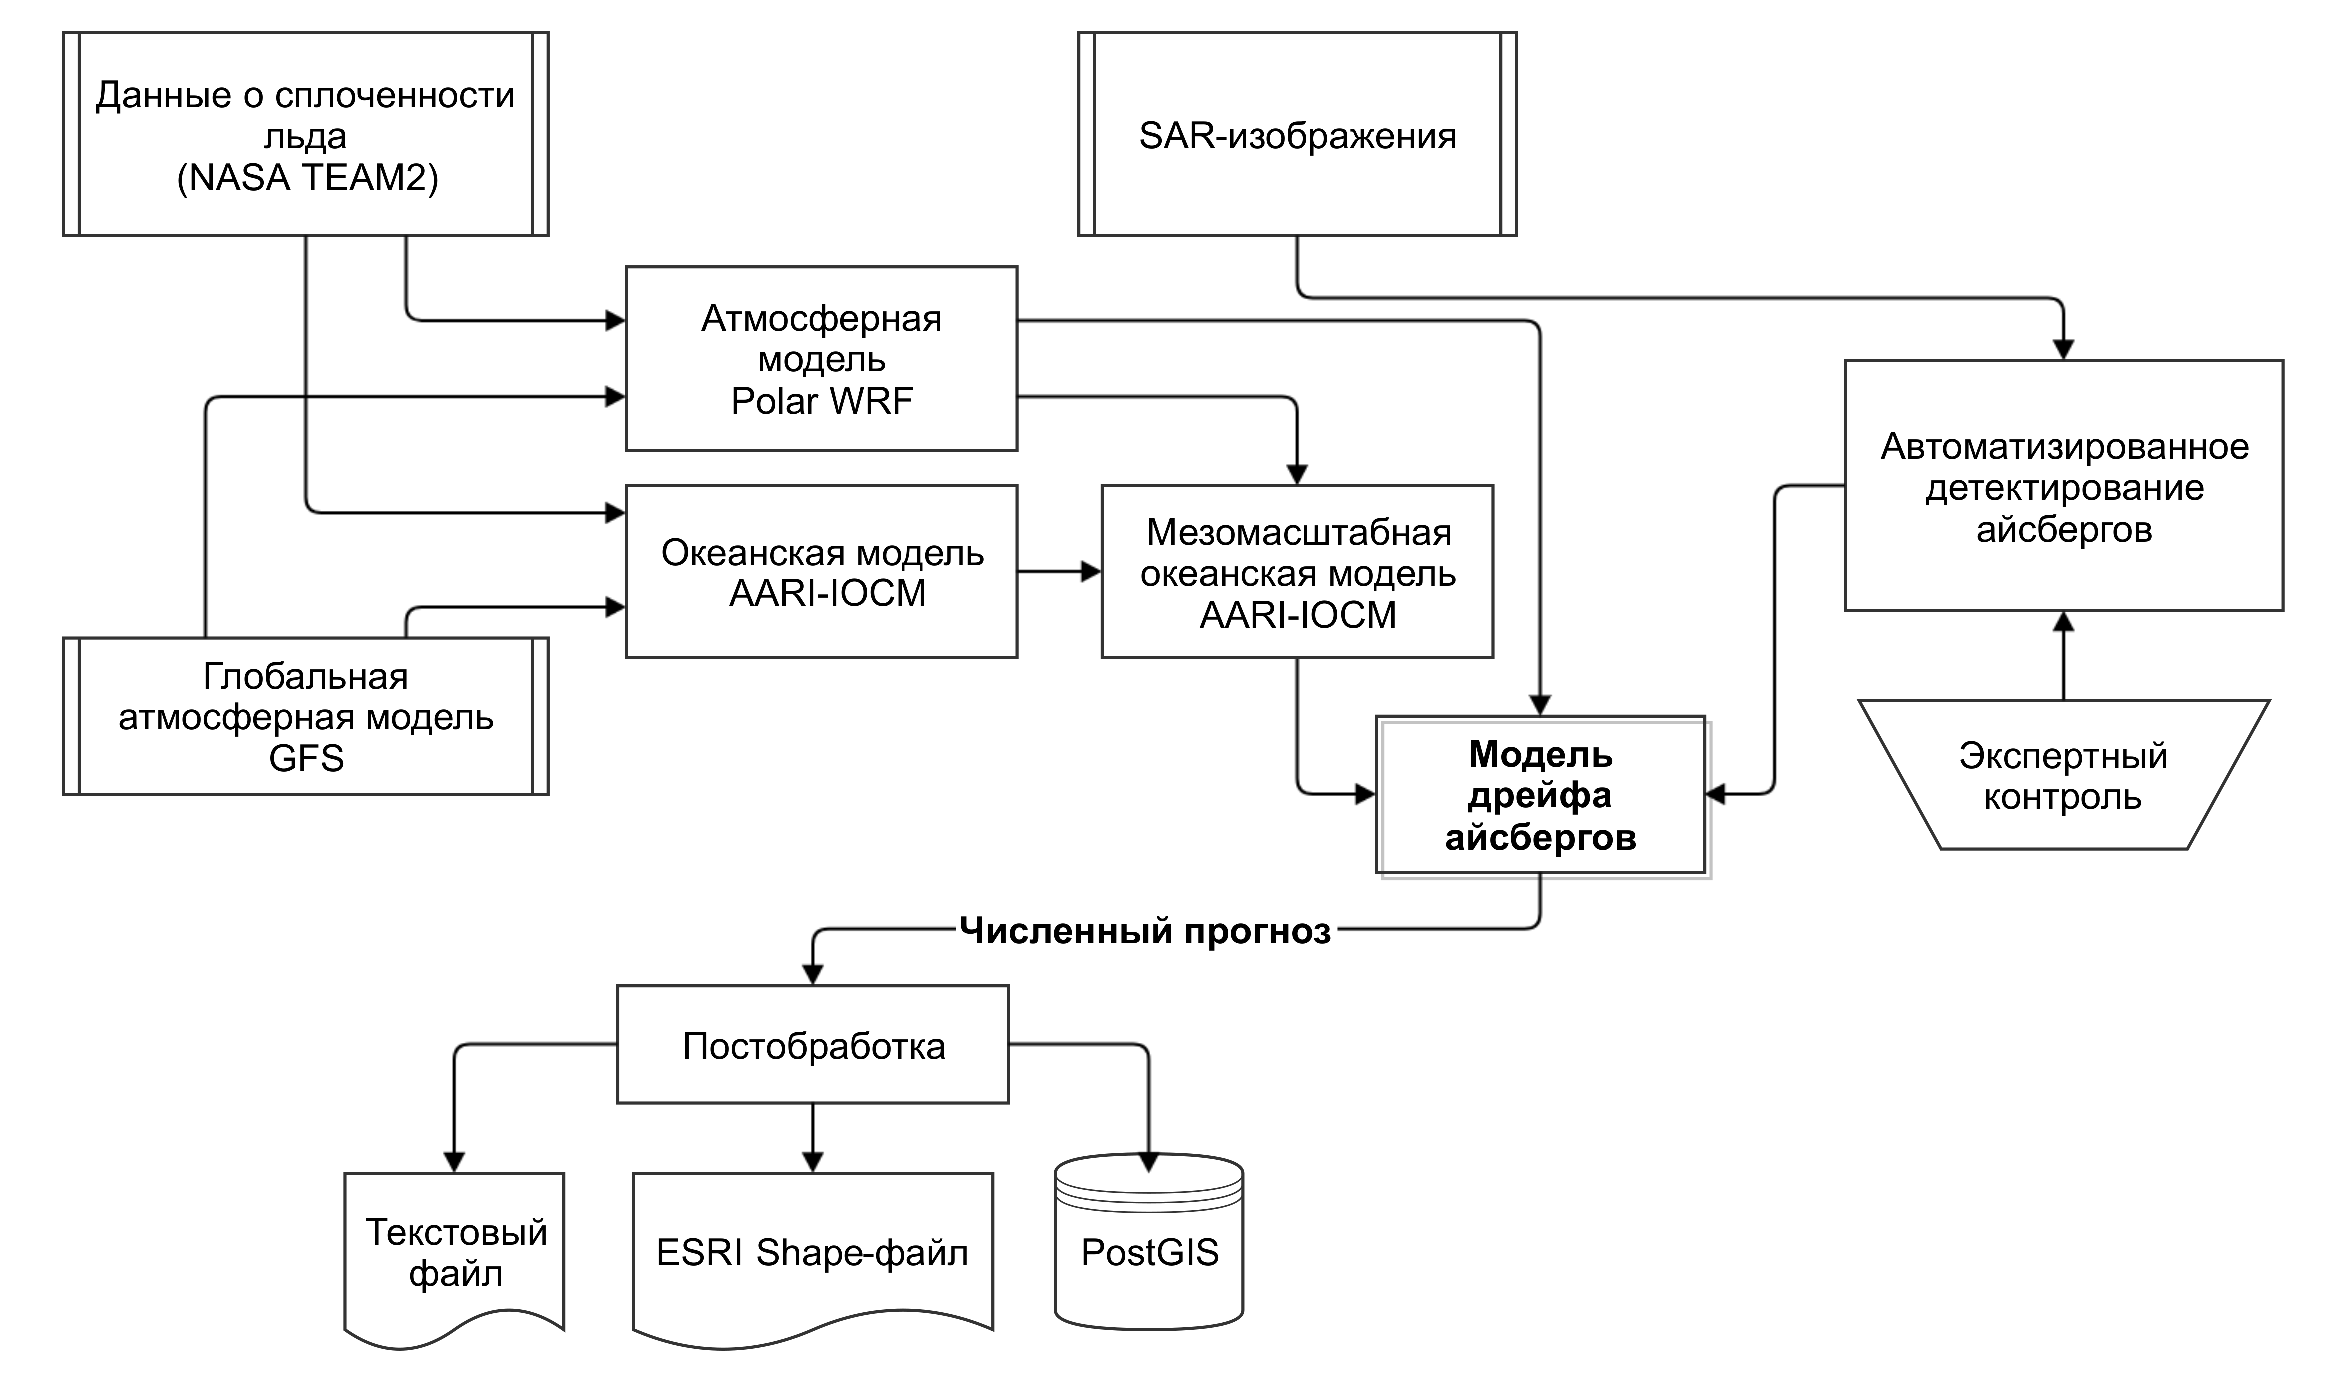
\includegraphics [scale=0.45] {iceberg_monitoring_scheme}
	\caption{Схема разработанной технологии мониторинга дрейфа айсбергов.}
	\label{img:iceberg_monitoring_scheme}
\end{figure}

В технологии можно выделить ряд крупных технологических блоков, или составляющих. 

\verb|Подготовка исходных данных|. В этот блок включены процедуры поступления
и преобразования входных данных к форматам, позволяющим обеспечить ввод этой
информации в модель. К этим данным относятся:

\noindent Маркированный список:
\begin{itemize}
	\item географические координаты о местоположении айсбергов полученные на основе метода обнаружения айсбергов по SAR"~данным высокого разрешения.
	\item данные глобальной атмосферной модели GFS, с горизонтальным разрешением 	сетки $0,5^\circ \times 0,5^\circ$. Данные скачиваются ежедневно с официального сайта NOAA~\footnote{\url{http://nomads.ncdc.noaa.gov/}}.
	\item гридированные данные о сплоченности морских льдов по данным пассивного микроволнового зондирования, с использованием прибора SSMI, на основе
	алгоритма NASATEAM (NT2)~\footnote{\url{ftp://sidads.colorado.edu/pub/DATASETS/nsidc0081_nrt_nasateam_seaice/north/}}.
\end{itemize}

\verb|Расчеты на глобальной модели AARI|"~\verb|IOCM|. Производится расчет всех элементов ледово"~гидрологического состояния СЛО на период используемого метеорологического прогноза GFS. С временной дискретностью 1 ч выводятся значения полных потоков на границах сеточной области региональной модели AARI"~IOCM.  

\verb|Расчеты на региональной модели WRF|. Для лучшего воспроизведения атмосферного форсинга в модельный комплекс включена атмосферная региональная модель WRF. В настоящий момент версия модели Polar~ WRF~\cite{bromwich2009development} адаптирована для района, покрывающего Юго"~Западную часть Карского моря и Печорское море с горизонтальным разрешением 4 км. Инициализация Polar~WRF происходит раз в сутки в 00 часов по Гринвичу, на основе данных глобальной модели GFS. В качестве данных о подстилающей поверхности используются результаты восстановления сплоченности морского льда на основе данных обработки пассивного микроволнового зондирования. В процессе расчетов выводятся значения атмосферного давления, приведенного к уровню моря, компонент скорости ветра и температуры воздуха на высоте 2 м с временной дискретностью 1 ч. Эти результаты используются для расчетов по региональной модели AARI"~IOCM.

\verb|Расчет на региональной модели AARI|"~\verb|IOCM|. Производится расчет всех элементов ледово"~гидрологического состояния на период используемого метеорологического прогноза. С временной дискретностью 6 ч выводятся значения составляющих скорости течения на 8 горизонтах (2,5; 7,5; 15; 25; 40; 62,5; 87,5 и 112,5 м), уровень моря, составляющие скорости ветра, толщина и сплоченность льда, а также составляющие скорости его дрейфа. Все выведенные результаты хранятся в файлах, с названиями, содержащими название параметра и время, которому они соответствуют.

\verb|Инициация модели дрейфа айсбергов|. На этом этапе формируется файл, содержащий информацию по айсбергам, для которых будут проводиться расчеты. В этом файле содержится информация о количестве айсбергов, их номера, время фиксации координат, координаты, длина, ширина, высота, осадка и масса каждого айсберга, указываются пути к директориям с входной информацией и местам хранения результатов расчетов.

\verb|Расчет на модели дрейфа айсбергов|. Модель дрейфа айсбергов реализована в лагранжевой постановке, поэтому значения всех необходимых для расчета форсингов ледово"~гидрологических параметров интерполируются в точку с координатами айсберга. После расчета величин всех сил, действующих на айсберг, численно решается дифференциальная задача об определении скорости дрейфа айсберга и определяются новые координаты айсберга. После этого вся процедура повторяется и так до достижения времени окончания прогноза. В результате расчетов по модели для каждого айсберга, участвовавшего в расчетах, формируется и записывается выходной файл, содержащий последовательность координат положений айсберга на каждые 6 часов (временной интервал может быть изменен в любую сторону) на весь период прогноза. Для уменьшения пространственного шага модели AARI"~IOCM использовалась процедура телескопирования, при которой на всей акватории СЛО используется обычный большой шаг (в нашем случае 13,8 км), а на акватории, для которой проводится прогнозирование, в несколько раз меньше. Для акватории Карского моря шаг модели составляет 4,6 км.

\verb|Постобработка результатов расчетов|. С помощью скриптов постобработки
на языке Python формируются линейные шейп"~файлы, которые являются конечным 
продуктом технологической цепочки. Эти файлы позволяют потребителям информации оперативно просматривать результаты расчетов, а также контролировать качество расчетов. Кроме того, ведется параллельная запись в геопространственную базу данных PostGIS.

Технология численного гидродинамического прогноза дрейфа айсбергов была успешно апробирована при оперативном обеспечении геологоразведочных работ на шельфе Карского моря. В течение августа "--- октября 2014 г. осуществлялось разведочное бурение на геологической структуре <<Университетская"~1>> на лицензионном участке Восточно"~Приновоземельский"~1 в Карском море. Бурение производилось морской полупогружной плавучей буровой установкой (ППБУ) <<West Alpha>>, не имеющей ледового класса, что обусловило повышенные требования к ее ледовому и гидрометеорологическому обеспечению. Специалисты Арктического и Антарктического Научно"~Исследовательского Института (<<ААНИИ>>) осуществляли полный комплекс работ по мониторингу окружающей среды и гидрометеорологическому обеспечению руководства морской операцией и капитана ППБУ. Главной задачей ледового мониторинга было обнаружение опасных ледяных образований (ледяные поля, несяки, айсберги), предсказание их дрейфа и возможного их столкновения с ППБУ. Также принималась во внимание возможность выноса с выводных ледников архипелага Новой Земли айсбергов и их обломков в район Университетской структуры~\cite{Mironov_Smirnov_Iceberg_2015}.

Прогноз дрейфа айсбергов заблаговременностью 24"--~72 часов готовился практически ежедневно и передавался, в основном, в формате шейп"~файлов в Береговой Операционный Центр (SOC "--- Shore Operational Center), который находился в Москве. В SOC вся информация анализировалась и передавалась на ППБУ и вспомогательные суда. Пример представления прогноза дрейфа айсбергов для потребителя представлен на рис.~\ref{img:ibg_frc}.

\begin{figure}[ht] 
	\centering
	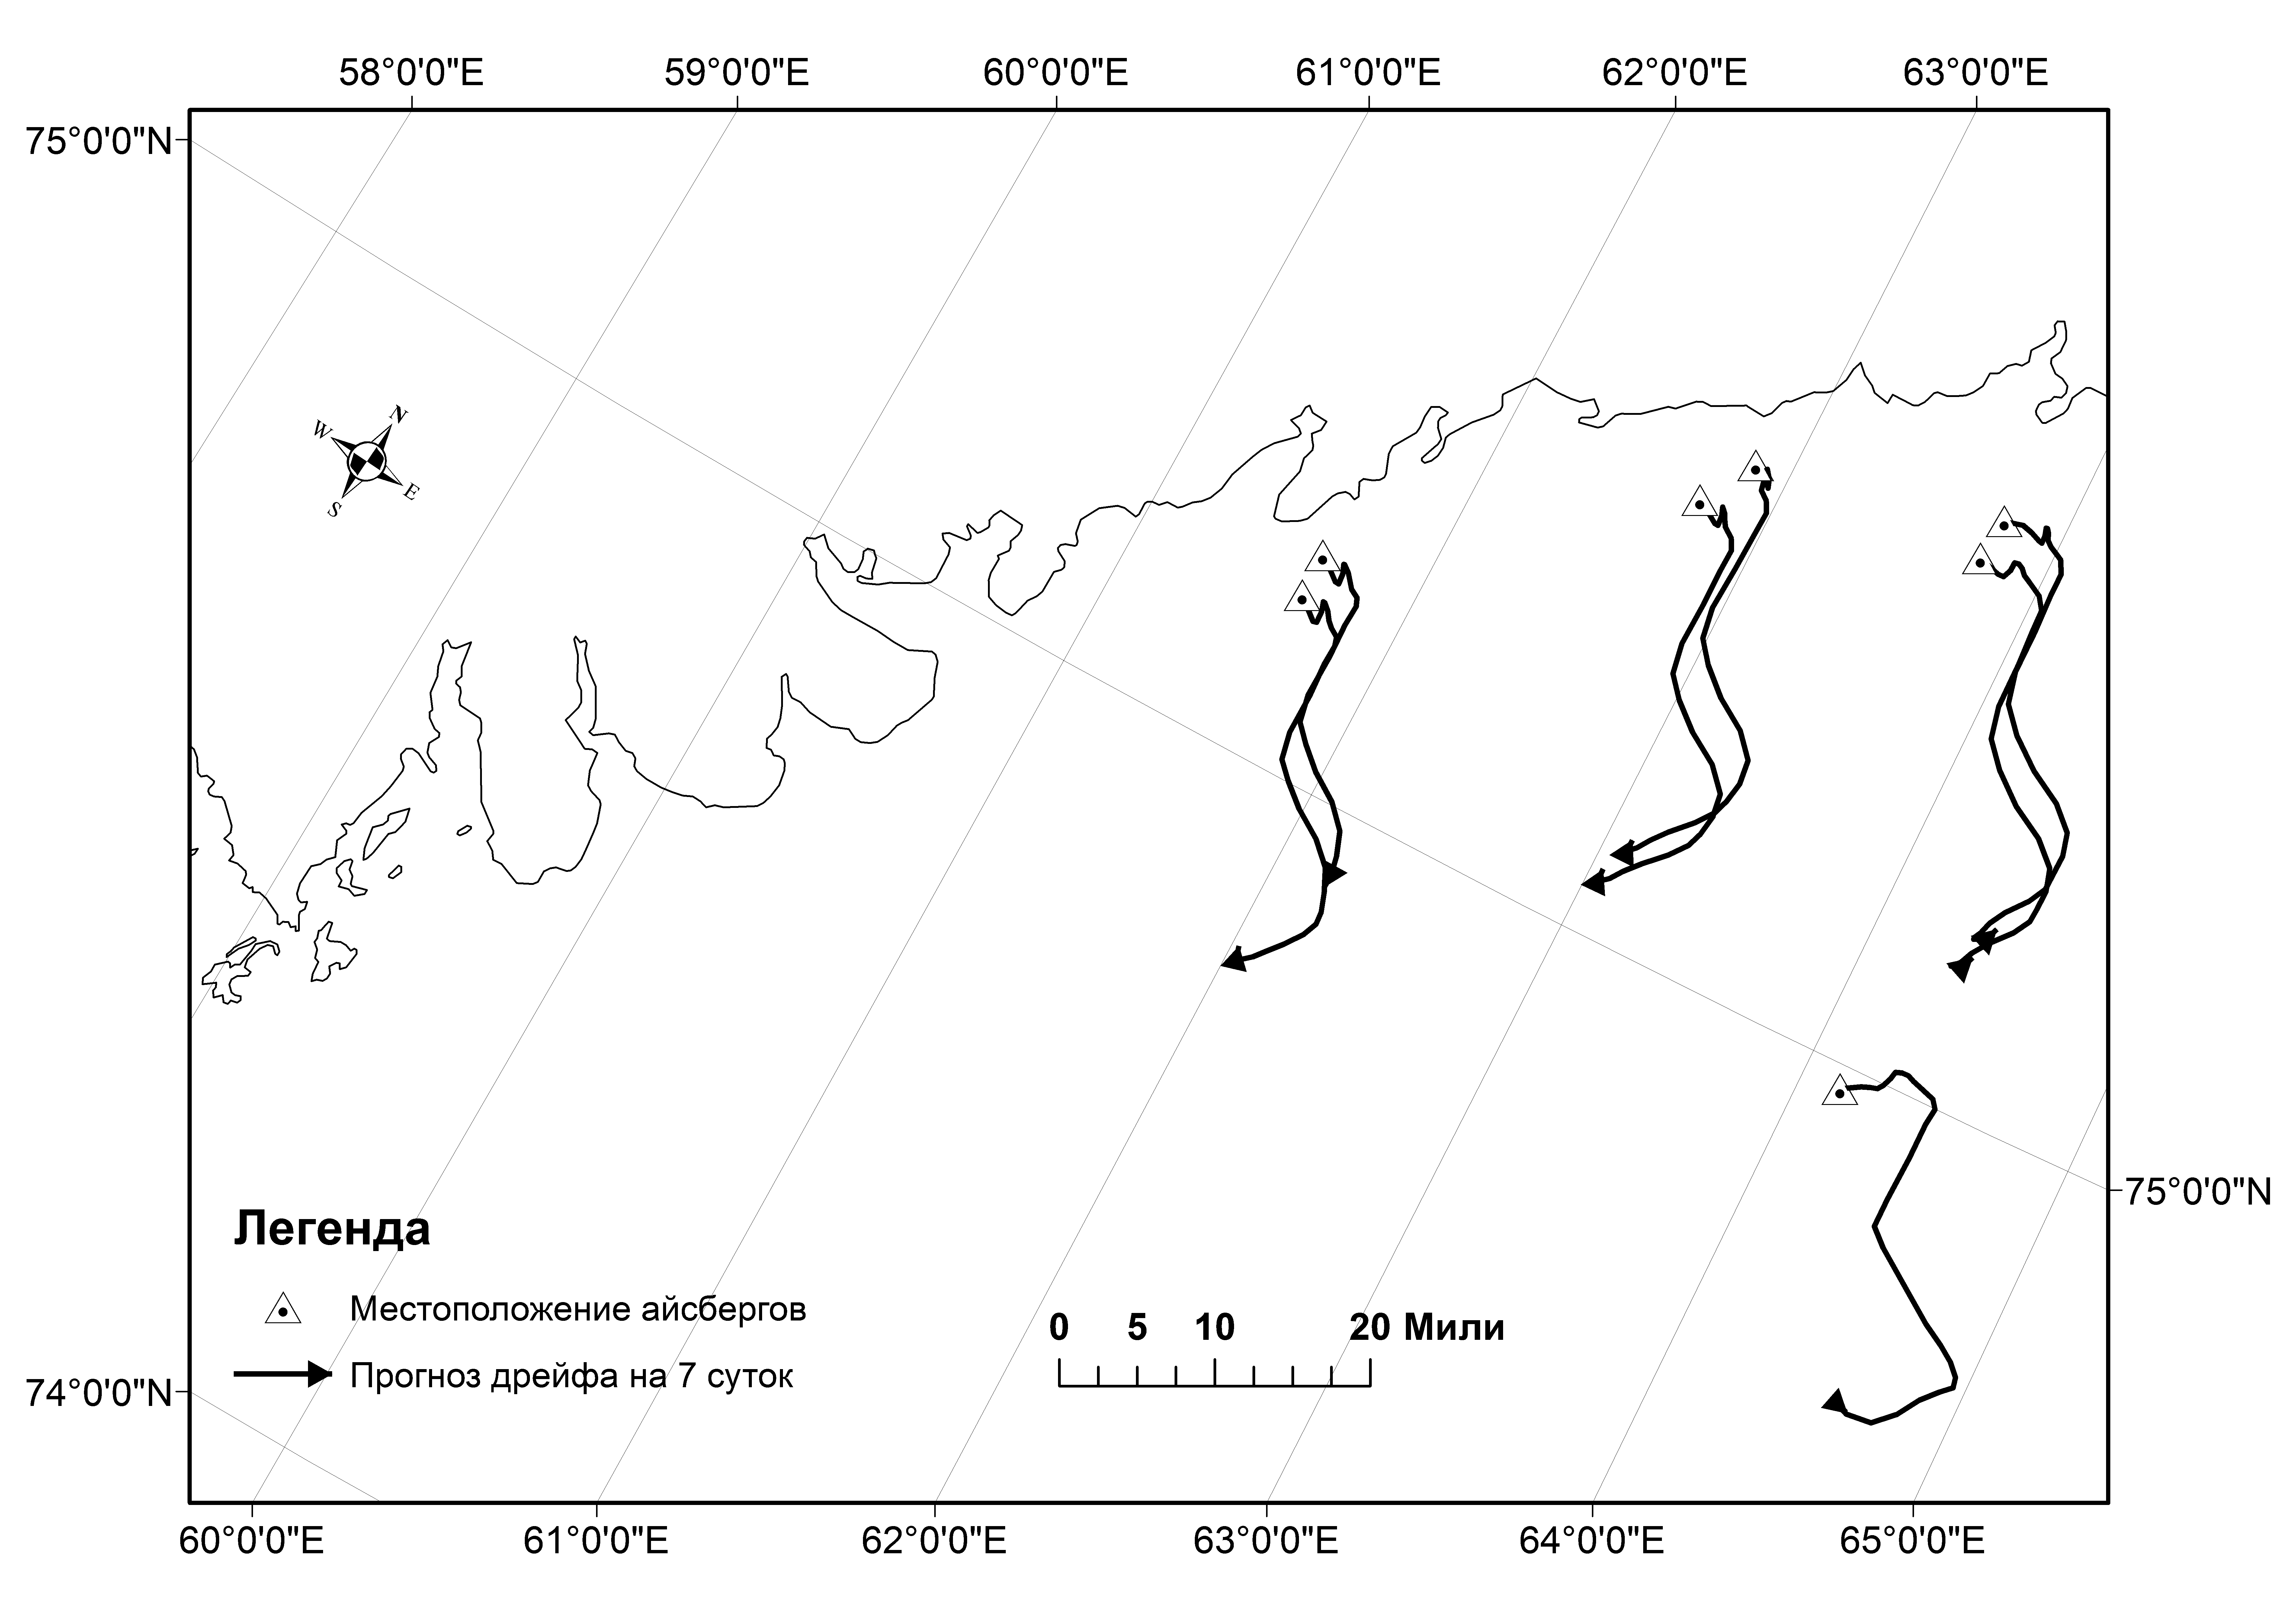
\includegraphics [scale=0.57] {ibg_frc}
	\caption{Пример прогноз дрейфа айсбергов на 09.09.2014, предоставленный в рамках ледового и гидрометеорологического обеспечения буровых работ в Карском море.}
	\label{img:ibg_frc}
\end{figure}

Оправдываемость и эффективность ледовых и гидрометеорологических прогнозов отвечала всем критериям действующих нормативных документов.

Гидрометеорологическое и ледовое обслуживания разведочного бурения в Карском море в 2014 г. обеспечило безопасность и эффективность работ, что способствовало открытию нового нефтяного месторождения <<Победа>>.

\subsection{Реконструкция дрейфа айсбергов в район ШГКМ в 2003 г.}\label{subsect4_1_3}
Для добычных комплексов на Штокмановском газоконденсатном месторождении (ШГКМ) в Баренцевом море наиболее опасными ледяными образованиями будут дрейфующие айсберги. По данным наблюдений за периоды 1928"--~1992 и 2002"--~2005 гг. на акватории, прилегающей к ШГКМ, было зафиксировано 220 айсбергов и кусков айсбергов~\cite{zubakin2007results}. Эти фиксации были отмечены в 1967, 1968, 1971, 1975, 1981, 1986, 1987, 1989, 1991 и 2003 г. 

Источниками айсбергов, распространяющихся на акватории Баренцева моря, являются арктические архипелаги Шпицберген, Земля Франца"~Иосифа, Новая Земля (о. Северный) и некоторые арктические острова (о. Ушакова и о. Виктория) и, даже Северная Земля~\cite{Koryakin1988,sandford1955tabular}. Важной составляющей ледового мониторинга является задача своевременного обнаружения айсбергов, потенциально опасных для добывающей платформы. Эта задача может быть успешно решена только в том случае, когда все источники айсбергов будут ранжированы по степени их угрозы.

За прошедшие годы было предпринято несколько попыток использовать математическое моделирование для оценки айсберговой опасности. Так, в~\cite{johannessen1999simulation} приводятся результаты модельных расчетов дрейфа айсбергов от южного побережья архипелага Земля Франца"~Иосифа. Авторы рассчитали траектории 3000 айсбергов стартовавших в июле, августе и сентябре за период от 1987 по 1996 гг. Согласно их результатам, ни один айсберг не достиг района ШГКМ. Большинство айсбергов дрейфовало на запад к архипелагу Шпицберген, некоторое количество айсбергов уходило в Центральный Арктический бассейн и только несколько дрейфовало на восток к северной оконечности Новой Земли.

Наблюдения за айсбергами выполненные в рамках экспедиции <<ШТОКМАН"~ЗИМА"~2003>>~\cite{Naumov2003}, когда непосредственно через площадь ШГКМ продрейфовало 104 айсберга и их обломков, свидетельствовали об обратном. По некоторым косвенным признакам айсберги, обнаруженные в районе ШГКМ, происходили от ледников архипелага Земля Франца"~Иосифа. 

В работе~\cite{Buzin2008} была предпринята попытка использовать моделирование для подтверждения гипотезы о том, что айсберги, обнаруженные в 2003 г. в районе ШГКМ, поступили туда от архипелага Земля Франца"--~Иосифа. Для этого была выполнена серия расчетов на гидродинамической модели~\cite{polyakov1998coupled} с подключенным к ней блоком перемещения айсбергов~\cite{Dmitriev1995}.

Начальной точкой выброса айсбергов являлась область в окрестностях Земли Вильчека (остров в архипелаге Земли Франца"~Иосифа), ледник которого предположительно является продуцентом крупных айсберговых образований, представляющих наибольшую угрозу для технических сооружений в открытой части Баренцева моря. Координаты данной точки: $\varphi=79,72184^\circ$ с.ш., $\lambda=53,36120^\circ$ в.д. Исходя из предпосылки о времени выброса, датированной окончанием летнего периода, за точку начального отсчета выбрано 1 сентября 2002 г. Общая продолжительность расчетов "---~ 8 месяцев (с 01.09.2002 по 30.05.2003). Модельный эксперимент проводился для 10 айсбергов с массой от 9,6 до 8150,5  тыс.\:т.

Модельные расчеты показали, что дрейф крупных айсбергов (с массой более 100 тыс.\:т), образовавшихся из ледников архипелага Земля Франца"~Иосифа в сентябре 2002 г., происходил преимущественно в юго"~западном и южном направлениях, и существовали все предпосылки к проникновению данных объектов в район ШГКМ, где они и были зафиксированы в мае 2003 г., в ходе выполнения экспедиционных работ <<ААНИИ>>.

В данной работе с помощью модели AARI"~IOCM была решена обратная задача. Для этого время было пущено вспять, а рассчитанные по модели приращения координат айсбергов не прибавлялись, а вычитались из предшествующих координат.

Расчеты на период май 2003 г. "--- май 2002 г. проводились для 12 айсбергов (таблица), морфометрические размеры которых были определены в рамках экспедиции «ШТОКМАН"~ЗИМА"~2003».

\begin{table} [htbp]%
	\centering
	\caption{Сводная таблица айсбергов, исследованных в 2003 г. в районе ШГКМ}%
	\label{tbl:tbl_icbergs_shtockman_2003}% label всегда желательно идти после caption
	\renewcommand{\arraystretch}{1.5}%% Увеличение расстояния между рядами, для улучшения восприятия.
	\setlength{\tymax}{1.9cm}
	\begin{SingleSpace}
		\begin{tabular}{@{}@{\extracolsep{0pt}}llllllllll@{}} %Вертикальные полосы не используются принципиально, как и лишние горизонтальные (допускается по ГОСТ 2.105 пункт 4.4.5) % @{} позволяет прижиматься к краям
			\toprule     %%% верхняя линейка
			Номер & Дата & Широта & Долгота & Длина & Ширина & Высота & Масса & Осадка &\\
			      &      & $^\circ$ с.ш. & $^\circ$ в.д. & м & м & м & кг & м &\\
			\midrule %%% тонкий разделитель. Отделяет названия столбцов. Обязателен по ГОСТ 2.105 пункт 4.4.5 
			%Прямоугольное 	& 8.72 	 & 8.77		& 8.77		\\
			
			1	&14.05	&74,590	&41,627	&40	&36	&6	&51	&50\\
			2	&13.05	&73,067	&41,132	&51	&44	&4	&52	&30\\
			3	&13.05	&73,028	&40,552	&52	&28	&5	&59	&40\\
			4	&14.05	&74,590	&41,610	&68	&43	&5	&108	&50\\
			5	&14.05	&74,588	&41,637	&107 &105	&4	&229	&40\\
			6	&14.05	&74,560	&41,200	&140 &86	&5	&394	&80\\
			7	&14.05	&74,690	&42,112	&135 &90	&4	&410	&40\\
			8	&14.05	&74,660	&42,100	&129 &97	&4	&427	&60\\
			9	&14.05	&74,630	&41,955	&190 &136	&5	&667	&40\\
			10	&14.05	&74,638	&41,903	&205 &180	&9	&1846	&100\\
			11	&13.05	&73,058	&41,325	&424 &190	&7	&3246	&60\\
			12	&14.05	&74,438	&41,530	&330 &160	&9	&3670	&90\\
			
			
			\bottomrule %%% нижняя линейка
		\end{tabular}%
	\end{SingleSpace}
\end{table}

Для удобства анализа и наглядности результаты расчетов обратного дрейфа айсбергов сгруппированы по четырем градациям массы: менее 60 тыс.\:т (а), от 100 до 400 тыс.т (б), от 400 до 700 тыс.\:т. (в) и свыше 1 млн.\:т. (г).

На рис. 3 представлены рассчитанные траектории обратного дрейфа айсбергов в 2003 – 2002 гг. от района ШГКМ. Траектории представлены последовательностью точек, фиксирующих положение айсберга через каждые шесть часов.

\begin{figure}[ht] 
	\centering
	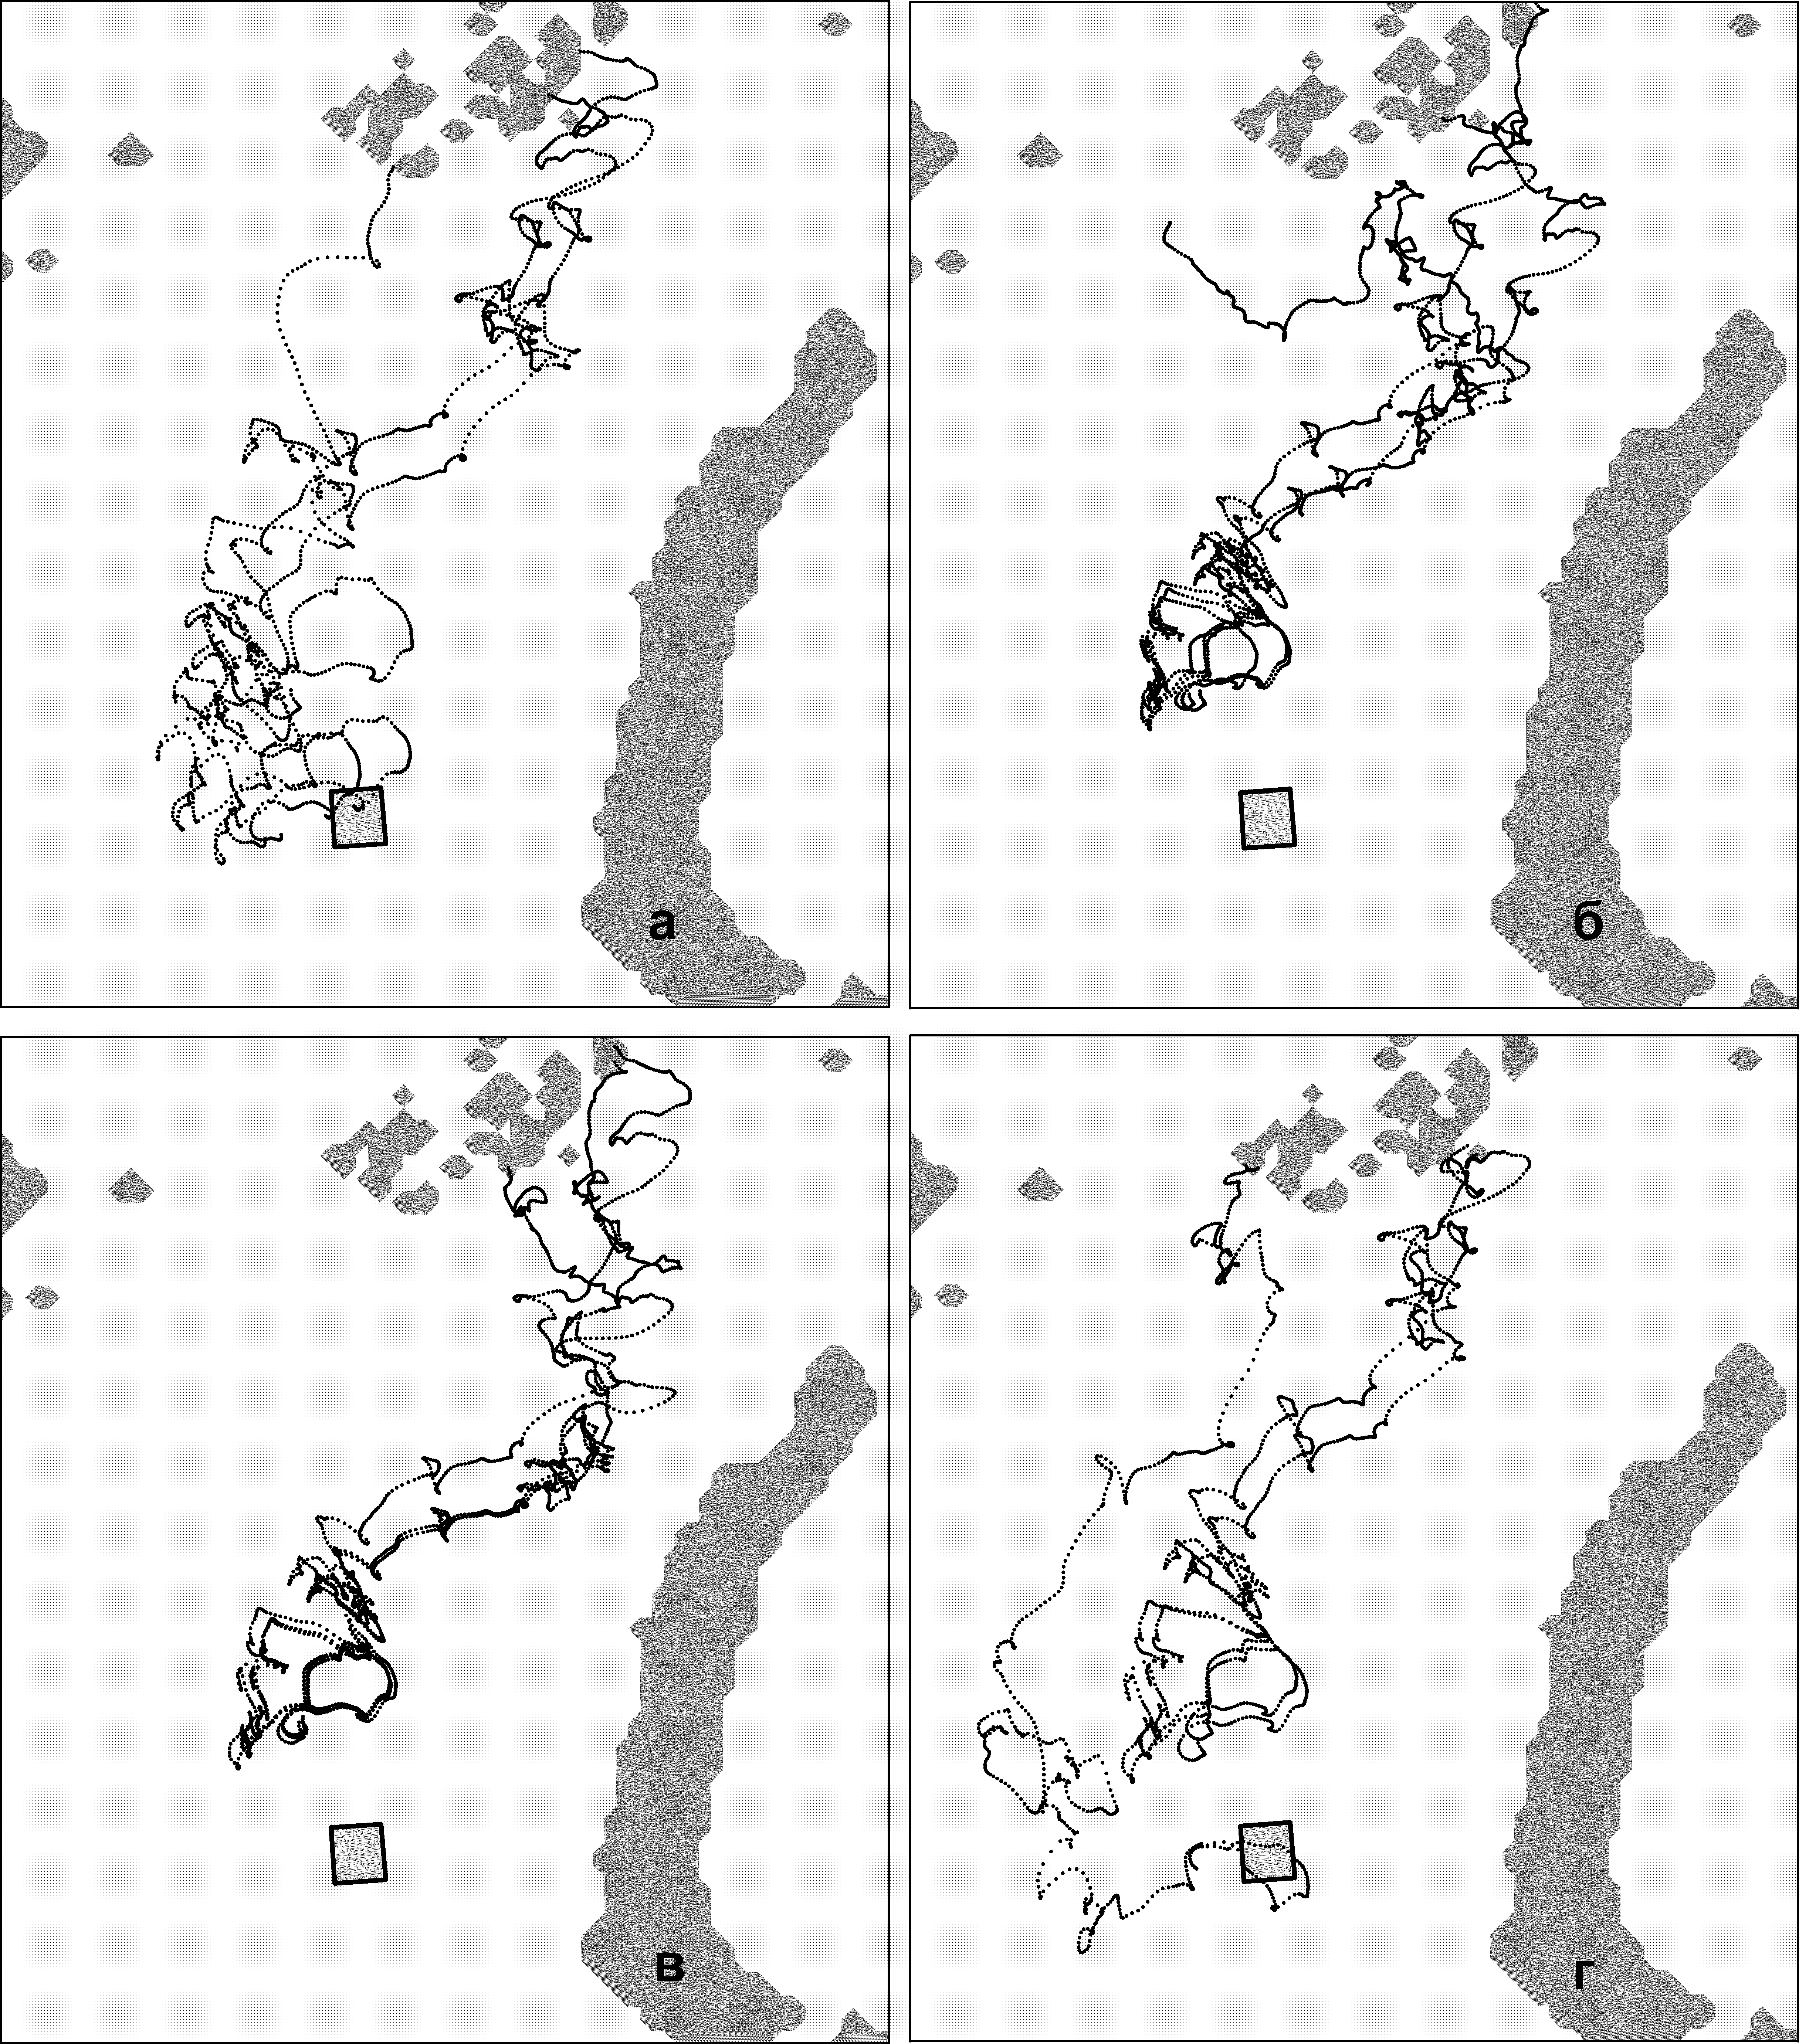
\includegraphics [scale=0.07] {ibg_frc_shtk}
	\caption{Рассчитанные траектории обратного дрейфа айсбергов в 2003"--~2002 гг. от района ШГКМ для категорий: менее 60 тыс.т (а), от 100 до 400 тыс.т (б), от 400 до 700 тыс.т. (в) и свыше 1 млн.т. (г).}
	\label{img:ibg_frc}
\end{figure}

Результаты продемонстрировали, что все айсберги, обнаруженные и измеренные в рамках экспедиции <<ШТОКМАН"~ЗИМА"~2003>> пришли в район ШГКМ от архипелага Земля Франца"~Иосифа. В первую очередь, следует отметить, что, несмотря на широкое многообразие морфометрических особенностей и масс айсбергов, большая часть их траекторий (9 из 12) закончилась у юго-восточного побережья архипелага, подтвердив тем самым предположение авторов~\cite{Buzin2008} о том, что наиболее вероятном источником айсбергов, могущих достигнуть район ШГКМ, является ледник на Земле Вильчека.

Время дрейфа айсбергов от побережья архипелага Земля Франца-Иосифа до района ШГКМ по результатам расчетов составило: для самого малого айсберга №1 "--- 5 месяцев, для остальных айсбергов "--- от 7 до 10 месяцев. Таким образом, наиболее благоприятным для достижения айсбергами района ШГКМ является период июль "--- октябрь. Не противоречит это и наблюдавшейся в 2002 г. ледовой обстановке вокруг архипелага Земля Франца"~Иосифа. В начале июля все южное побережье уже было свободно не только от дрейфующих льдов, но и от припая.

Таким образом, выполненные модельные эксперименты показали, что ледники архипелага Земля Франца"~Иосифа являются наиболее вероятным источником айсбергов, опасных для добывающей платформы на ШГКМ. Время достижения айсбергами района ШГКМ составляет от 7 до 10 месяцев, но возможно и более быстрое продвижение. Все это необходимо учитывать при разработке системы мониторинга айсбергов на акватории Баренцева моря.

\subsection{Выводы}\label{subsect4_1_4}
Разработана технология мониторинга дрейфа айсбергов на основе численной гидродинамической модели, с использованием автоматизированного анализа данных  спутниковых радиолокаторов высокого разрешения, которая может использоваться для решения целого ряда задач в системе мониторинга ледовой обстановки в Западной Арктической зоне Российской Федерации.

Численные эксперименты на модели позволили получить важные закономерности распространения айсбергов в Баренцевом море, которые будут востребованы при оптимизации системы мониторинга в Западной Арктике.

Оперативное применение модели для производства краткосрочных прогнозов (24"--~72 часа) для гидрометеорологического обеспечения разведочного бурения на геологической структуре «Университетская"~1» на лицензионном участке Восточно"~Приновоземельский"~1 в Карском море в 2014 г. продемонстрировало эффективность разработанной технологии, которая может стать важными блоком при создании автоматизированной системы управления ледовой обстановкой в арктических морях.

\newpage
%============================================================================================================================

\section{Мониторинг динамических характеристик льда "--- дрейфа и деформации в районе судоходного канала Обской губы} \label{sect4_2}

В данном параграфе приводится описание технологии расчета дрейфа льда на основе разработанного алгоритма (см. Главу~\ref{chapt2}) и ее применение для мониторинга динамических характеристик льда "--- дрейфа и деформации на примере района прилегающего к судоходному каналу Обской губы. В качестве входной информации используются данные спутников Sentinel"~1A/B и Radarsat"~2.

\subsection{Технология расчета дрейфа льда} \label{subsect4_2_1}

\subsection{Технология расчета деформационных характеристик льда} \label{subsect4_2_2}

Описание пространственных градиентов полей дрейфа льда "--- деформационных характеристик, имеет важное значение для понимания процессов взаимодействия в системе атмосфера"~океан"~лед и адекватного описания морского льда в численных моделях для решения задач прогнозирования его состояния в будущем. Это особенно актуально в районах с развивающейся газо"~нефте добычей, таких как Обская губа. В современных исследованиях было показано, что результаты статистической обработки данных наблюдений не совпадают с данными полученными на основе численного моделирования, в частности "--- распределение скоростей деформации, а также закономерности ее изменчивости в зависимости от пространственного и временного масштабов~\cite{girard2009evaluation}, за воспроизведение которых отвечает блок механики льда. В ~\cite{girard2009evaluation} делается вывод что это несоответствие может быть вызвано некорректным описанием физико"~механических свойств льда. В работе Вейса~\cite{weiss2008intermittency} было показано, что характер возникающих во льду напряжений главным образом обусловлена механикой льда, а не ветровым форсингом. В данной работе показано, что в случае корректного описания физико"~механических свойств льда, воспроизведение динамических параметров будет близким к наблюденным даже в случае ветрового форсинга посредственного качества. Эти и ряд других исследований~\cite{2011ipcc,rampal2009positive} указывают на важность изучения деформационных характеристик на региональном масштабе для улучшения качества воспроизведения параметров морского льда, особенно процессов образования разводий и полыней, торошения льда в численных моделях что как следствие "--- будет способствовать повышению оправдываемости ледовых прогнозов.

Далее приводятся, полученные впервые, результаты расчетов динамических характеристик льда в акватории Обской губы на примере ледового сезона 2016"--~2017 гг.

\begin{figure}[ht] 
	\centering
	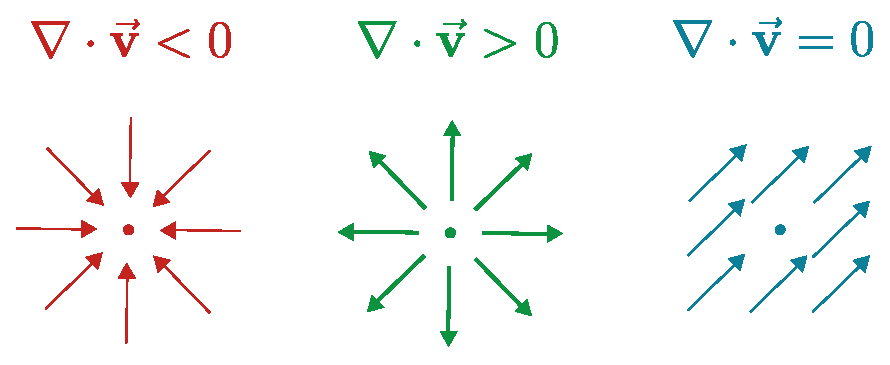
\includegraphics [scale=0.7] {divergence}
	\caption{Схематичное представление знака значений дивергенции при различных направлениях потока.}
	\label{img:divergence_example}
\end{figure}

%\newpage
%============================================================================================================================



\clearpage